\chapter{Analysis of Flutter}\label{ch:analysis-of-flutter}

This chapter describes the key reasons why Dronetag chose Flutter for the mobile application development.

Nowadays, many companies have more teams to maintain their application that ensure the companies' business.
Thanks that the costs are higher than could be and this is the reason why cross-platform frameworks were created.
There are many cross-platform mobile application platforms to develop an application like this.
The name of the main used frameworks are:
\begin{itemize}
    \item React Native,
    \item Ionic and
    \item Xamarin.
\end{itemize}

Flutter is a framework and was established by Google Inc., in 2017 and since that time, its popularity is still increasing.

React Native looks like the main competitor and is based on JavaScript.\cite{flutterVsReactNativeNevercodeIo}
Ionic has not a such good performance like Flutter and React Native.
Xamarin is based on C\# from Microsoft and thus we avoided it.
Flutter is based on Dart which was introduced by Google Inc., in 2011.
It is type safe and object oriented programming language similar to Java.\cite{dartTypeSystem}
Between advantages of Flutter belong:
\begin{itemize}
    \item Hot Reload, i.e., allows fast coding,
    \item One codebase: Development for two mobile platforms,
    \item Up to 50\% less testing,
    \item Faster app development,
    \item User-friendly designs,
    \item Perfect for MVPs and
    \item Less Code.\cite{flutterVsReactNativeHackrIo}
\end{itemize}

\section{General concept}\label{sec:general-concept}
"Flutter is an app SDK for building high-performance, high-fidelity apps for iOS, Android, web (beta), and desktop (technical preview) from a single codebase."\cite{flutterTechnicalOverview}
It means you need only one development team to reach an application for all platform in a single codebase.

"The goal is to enable developers to deliver high-performance apps that feel natural on different platforms.
We embrace differences in scrolling behaviors, typography, icons, and more."\cite{flutterTechnicalOverview}

%TODO: add some words of mine

\begin{figure}
    \centering
    \begin{minipage}{.45\textwidth}
        \centering
        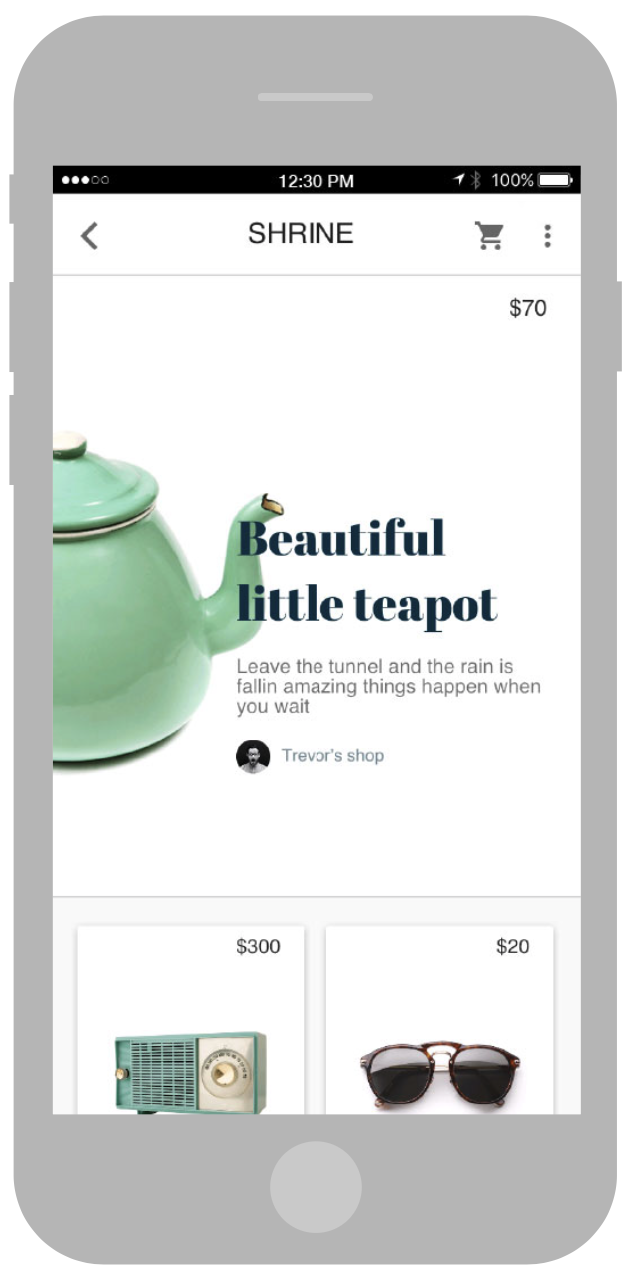
\includegraphics[width=.7\linewidth]{assets/hero-shrine-ios.png}
        \caption{Flutter demo app on iOS \cite{flutterTechnicalOverview}}
        \label{fig:flutter-demo-app-ios}
    \end{minipage}%
    \hspace{.05\linewidth}
    \begin{minipage}{.45\textwidth}
        \centering
        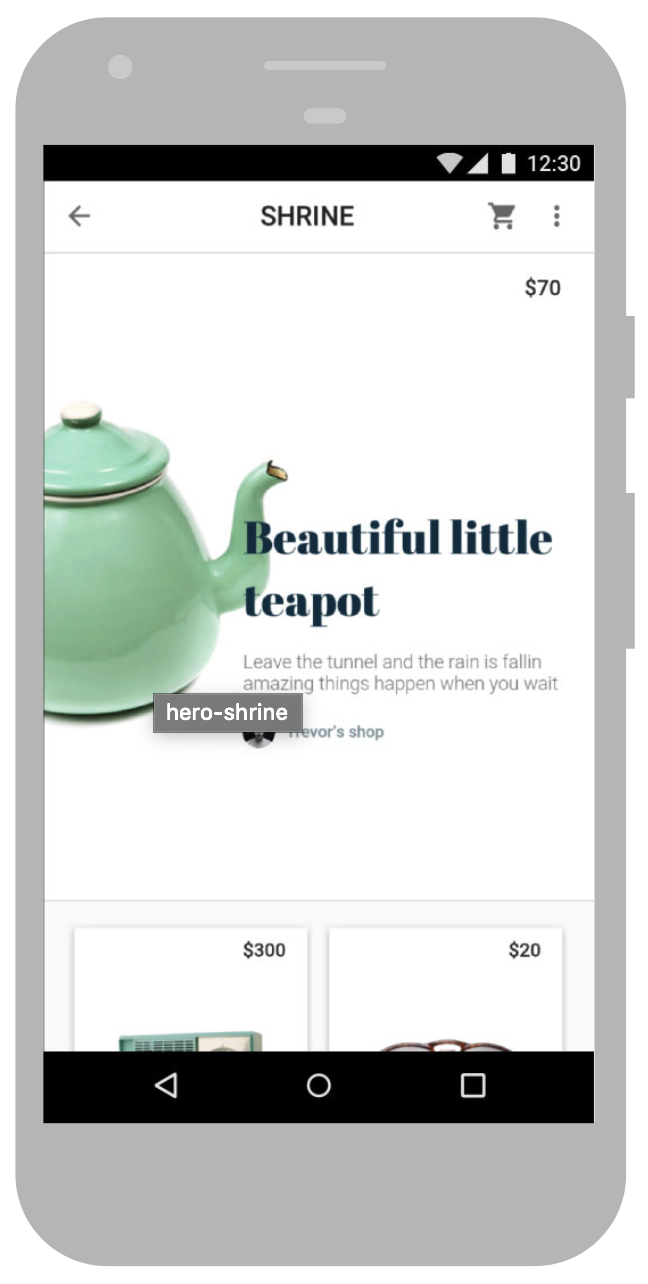
\includegraphics[width=.7\linewidth]{assets/hero-shrine-android.png}
        \caption{Flutter demo app on Android \cite{flutterTechnicalOverview}}
        \label{fig:flutter-demo-app-android}
    \end{minipage}
    \label{fig:flutter-demo-app}
\end{figure}


\subsection{Flutter UI}\label{subsec:flutter-ui}
"Flutter includes a modern react-style framework, a 2D rendering engine, ready-made widgets, and development tools.
These components work together to help you design, build, test, and debug apps.
Everything is organized around a few core principles."\cite{flutterTechnicalOverview}
Flutter has a widget tree that renders widget into nested tree, and these widgets are covering themselves.
It does not matter if a widget from the widget tree is Container, List View, Image, Text, Animation or anything else.
Everything is represented by a widget or its descendents.

\section{Widgets}\label{sec:widgets}
How the founders of Flutter say: "Everything is a Widget".
In the following part, this statement will be clarified.

"Widgets are the basic building blocks of a Flutter app's user interface.
Each widget is an immutable declaration of part of the user interface.
Unlike other frameworks that separate views, view controllers, layouts, and other properties, Flutter has a consistent, unified object model: the widget.
A~widget can define:
\begin{itemize}
    \item A structural element (like a button or menu),
    \item A stylistic element (like a font or color scheme),
    \item An aspect of layout (like padding),
    \item And so on \textellipsis"~\cite{flutterTechnicalOverview}
\end{itemize}
So each component of UI in Flutter is a descendent of the widget.
There are many classes that inherit from a widget.
The essential descendants are the following:
\begin{itemize}
    \item StatelessWidget,
    \item StatefulWidget,
    \item InheritedWidget.
\end{itemize}


\subsection{StatelessWidget}\label{subsec:statelesswidget}
"A widget that does not require mutable state.
A stateless widget is a widget that describes part of the user interface by building a constellation of other widgets that describe the user interface more concretely.
The building process continues recursively until the description of the user interface is fully concrete (e.g., consists entirely of
\textit{RenderObjectWidgets}~\cite{renderObjectWidget}, which describe concrete \textit{RenderObjects}~\cite{renderObject})."~\cite{statelessWidget}
It means that StatelessWidget is a useful component to render graphics elements that do not change during their lives.
StatelessWidget is class with Constructor and build method.
When the widget tree is built, it calls the build method.

"Stateless widget are useful when the part of the user interface you are describing does not depend on anything other than the configuration information in the object itself and the BuildContext in which the widget is inflated.
For compositions that can change dynamically, e.g. due to having an internal clock-driven state, or depending on some system state, consider using StatefulWidget."~\cite{statelessWidget}


\subsection{StatefulWidget}\label{subsec:statefulwidget}
"A widget that has mutable state.
State is information that (1) can be read synchronously when the widget is built and (2) might change during the lifetime of the widget.
It is the responsibility of the widget implementer to ensure that the \textit{State}~\cite{state} is promptly notified when such state changes, using \textit{State.setState}~\cite{setState}."~\cite{statefulWidget}
It means that StatefulWidget is a useful component to render graphics elements that change until they are disposed of.
StatefulWidget initializes its state, which represents a space for storing data.
The State is class with constructor, initState and build method.
The constructor is called when the State is created.
The initState method is called before the widget tree is rendered, and the build method is called when the tree renders itself.

Due to this fact, the Stateful widget has worse performance than StatelessWidget, and often it is difficult to keep a sustainable design of a component.
On the other hand, it offers a convenient way to create a widget with few states that will not be changed in the future development cycle.

"Stateful widgets are useful when the part of the user interface you are describing can change dynamically, e.g. due to having an internal clock-driven state, or depending on some system state.
For compositions that depend only on the configuration information in the object itself and the BuildContext in which the widget is inflated, consider using StatelessWidget."~\cite{statefulWidget}


\subsection{InheritedWidget}\label{subsec:inheritedwidget}
"Base class for widgets that efficiently propagate information down the tree.

To obtain the nearest instance of a particular type of inherited widget from a build context, use \textit{BuildContext.dependOnInheritedWidgetOfExactType}~\cite{dependOnInheritedWidgetOfExactType}.

Inherited widgets, when referenced in this way, will cause the consumer to rebuild when the inherited widget itself changes state."~\cite{inheritedWidget}
It means that InheritedWidget is a useful component to pass data and offer to reduce boilerplate if there are many widgets nested in themselves.
Thanks to the BuildContext class and of a method, you can easily get the value you add as an input variable.
So it means the widget is suitable for passing a huge amount of data.
It loses a need to copy many parameters in a large tree structure.


\section{Bloc}\label{sec:bloc}
Bloc is an abbreviation of Business Logic Component and allows separating an application into separate layers.~\cite{bloc}
"The BLoC Pattern has been designed by Paolo Soares and Cong Hui, from Google and first presented during the DartConf 2018 (January 23--24, 2018)."~\cite{didierboelens}

"The goal of this package is to make it easy to implement the BLoC Design Pattern (Business Logic Component).

This design pattern helps to separate presentation from business logic.
Following the BLoC pattern facilitates testability and reusability.
This package abstracts reactive aspects of the pattern allowing developers to focus on converting events into states."~\cite{bloc}

Bloc is a library written by Felix Angelov and the concept bases on Reactive Programming.~\cite{bloc}
Bloc represents a control unit that is responsible for passing data from state into UI.
When a user clicks on a button, it throws an event action that Bloc detects and generates a new state.~\cite{bloc}
In a summary, a structure of the concept consists of the following parts in Bloc:
\begin{itemize}
    \item \textbf{Events} are the input to a Bloc.
    They are commonly UI events such as button presses.
    Events are added to the Bloc and then converted to States.
    \item \textbf{States} are the output of a Bloc.
    Presentation components can listen to the stream of states and redraw portions of themselves based on the given state (see BlocBuilder for more details).
    \item \textbf{Transitions} occur when an Event is added after mapEventToState has been called but before the Bloc's state has been updated.
    A Transition consists of the currentState, the event which was added, and the nextState.
    \item \textbf{BlocSupervisor} oversees Blocs and delegates to BlocDelegate.
    \item \textbf{BlocDelegate} handles events from all Blocs which are delegated by the BlocSupervisor.
    Can be used to intercept all Bloc events, transitions, and errors.
    It is a great way to handle logging/analytics as well as error handling universally.
\end{itemize}

\begin{figure}
    \centering
    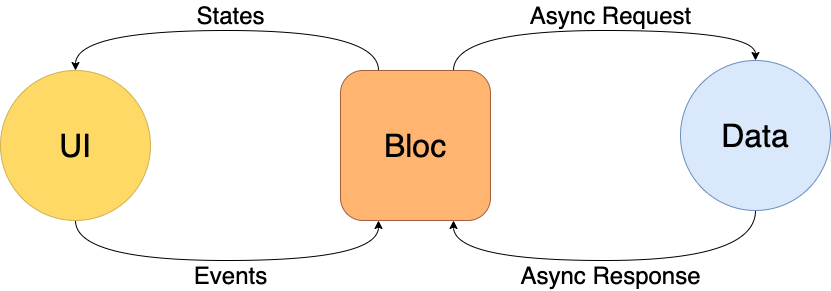
\includegraphics[scale=0.4]{assets/bloc_architecture.png}
    \caption{Bloc architecture~\cite{bloc}}
    \label{fig:bloc-architecture}
\end{figure}

\section{HydratedBloc}\label{sec:hydratedbloc}
"\textit{hydrated\_bloc}~\cite{hydratedBlocPubDev} is an extension to the \textit{bloc state management library}~\cite{bloc} which automatically persists and restores bloc states.

\textbf{hydrated\_bloc} exports a \textbf{HydratedStorage} interface which means it can work with any storage provider.
Out of the box, it comes with its own implementation: \textbf{HydratedBlocStorage}.

\textbf{HydratedBlocStorage} is built on top of \textit{path\_provider}~\cite{pathProvider} for a platform-agnostic storage layer.
The out-of-the-box storage implementation reads/writes to file using the \textbf{toJson/fromJson} methods on \textbf{HydratedBloc} and should perform very well for most use-cases (performance reports coming soon).
\textbf{HydratedBlocStorage} is supported for desktop (\textit{example}~\cite{hydratedBlocExample})."~\cite{hydratedBlocTut}

HydratedBloc works as well as common Bloc.
The difference is in data storage.
Hydrated Bloc allows us to store data through a JSON object.
So, whenever an application loads data, it is necessary to wait and show the user progress indicator, but it can show stored data immediately.
When it receives data, it will simply render it into a screen.

"\textbf{HydratedBlocStorage} is an implementation of \textit{HydratedStorage} which uses \textit{PathProvider} and \textit{dart.io} to persist and retrieve state changes from the local device."~\cite{hydratedBlocStorage}
So, it is a part of Hydrated Bloc implementation.

\section{iOS specific UI widgets - Cupertino library}\label{sec:ios-specific-ui-widgets}
Cupertino is a library ...


\section{Android specific UI widgets - Material Design}\label{sec:android-specific-ui-widgets}
Material Design is a concept that was introduced by Google company ...
